\documentclass[a4paper]{article}

\usepackage[english]{babel}
\usepackage[T1]{fontenc}
\usepackage[utf8]{inputenc}
\usepackage{amsmath}
\usepackage{graphicx}
\usepackage{lmodern}
\usepackage[left=3cm, right=3cm, bottom=4cm, top=4cm]{geometry}
\usepackage{array}
\usepackage{pdfpages}

\usepackage[gen]{eurosym}
\DeclareUnicodeCharacter{20AC}{\euro{}}

\usepackage{hyperref}
\hypersetup{    
    colorlinks,
    citecolor=black,
    filecolor=black,
    linkcolor=black,
    urlcolor=black
}


\title{Machine learning mini project - Data smashing}

\author
{
	Héctor {\sc Anadón León}\\
    Primož {\sc Godec}\\
    Hoel {\sc Kervadec}\\
    Tomáš {\sc Urbanec}
}

\date{\today}

\begin{document}
    \maketitle

    \begin{abstract}
        During the machine learning course at LTU, we had to implement a state of the art algorithm, called Data Smashing. The aim was to provide a easy to use implementation, usable on a web browser and plotting the results in a nice and readable way.

        We then used our work to analyze data from real world < and then what ? >.
    \end{abstract}
    
    % \setcounter{tocdepth}{2}
    \tableofcontents
    \setlength{\parskip}{10pt}
    
    \section{Introduction}
	During the machine learning courses at LTU, we had the occasion to implement state of the art tools

    \section{Data smashing}
	Data smashing\cite{data_smashing} is a new way to compare data stream from different stochastic sources, 

    \section{Our implentation}
	The goal was to provide an interface to easily select data and plot results.
	We decided to create a website, which can easily be deployed on a web server or on a personal computer
	To do so, we decided to use Python as primary language, and Django for the web part.

	\subsection{Development process}
		After creating a basic interface to provide and display input data, we started the implementation of the algorithm.
		To test our results, we used basic automata (as shown in figure \ref{fig:automata}), with some probability transitions, to generate data streams.
		This way, we were able to compare streams from the same automata, or different ones, and therefore validating our results.

		\begin{figure}
			\begin{center}
				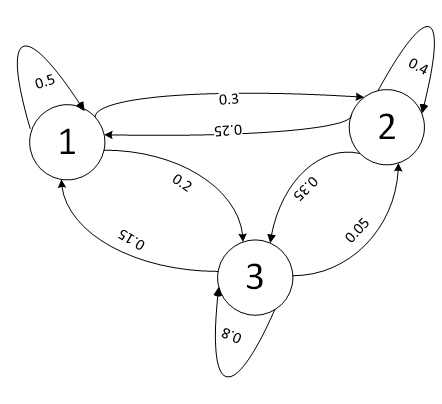
\includegraphics[width=0.8\textwidth]{figures/automata.png}
			\end{center}
			\caption{Example of an automata generating stream for us.}
			\label{fig:automata}
		\end{figure}

		Indeed, two streams from the same automata should have a deviation close to 0, when streams from differents automata should have a much higher deviation.

	

    \section{Our results}
	After validating our algorithms with generated data, we then moved to real world data.

    \section{Conclusion}
	We did it, yay.

    \bibliographystyle{plain}
    \bibliography{input/biblio}
\end{document}